\documentclass[12pt,a4paper]{article}
\usepackage[utf8]{inputenc}
\usepackage{polski}
\usepackage[polish]{babel}
\usepackage{amsmath}
\usepackage{amsfonts}
\usepackage{amssymb}
\usepackage{graphicx}
\usepackage{wrapfig}
\usepackage{caption}
\usepackage{mhchem}

\numberwithin{equation}{section}


\renewcommand{\baselinestretch}{1.5}
\captionsetup[figure]{labelformat={default},name={\bfseries Rys.}}
\captionsetup[table]{labelformat={default},name={\bfseries Tab.}}

\newcommand*{\captionsource}[2]{%
	\caption[{#1}]{%
		#1%
		\\\hspace{\linewidth}%
		\textbf{Żródło:} #2%
	}%
}


\title{3. Elektroliza}
\date{8 listopada 2017}	
\author{
	Zespół 3: Górski Paweł, Sozańska Ada\\
	EAIiIB Informatyka, Rok II
}

\begin{document}
\maketitle
% WPROWADZENIE
\section{Wprowadzenie}
Celem tego doświadczenia jest wyznaczenie wartości stałej Faradaya oraz ładunku elementarnego metodą elektrolizy dla soli \ce{CuSO4}.

\subsection{Elektroliza}

Elektroliza jest to proces zachodzący w układach zawierających substancje zdolne do jonizacji. Zjawisko to zostaje wywołane poprzez przyłożenie napięcia do elektrolitu przy użyciu elektrod. Sam elektrolit jest substancją zdolną do dysocjacji elektrolitycznej, czyli rozpadu na jony. Elektrolitami są między innymi roztwory wodne kwasów, zasad oraz soli. 

Różnica potencjałów na elektrodach wymusza przemieszczanie się jonów (nośników ładunku) w roztworze do elektrod o przeciwnych ładunkach. Jony dodatnie zwane są kationami, a ujemne anionami. W przypadku elektrod, katodami nazywamy elektrody o ładunku ujemnym, a anodami elektrody o ładunku dodatnim. W wyniku elektrolizy na elektrodach może wytrącać się osad (związek chemiczny lub pierwiastek), wydzielać gaz lub zachodzić reakcja chemiczna.

Masę wydzieloną na elektrodach można obliczyć, korzystając z \textit{Praw elektrolizy Faradaya}.

\subsection{Prawa elektrolizy Faradaya}

Pierwsze prawo elektrolizy dotyczy proporcjonalności masy. Mówi ono, że masa $m$ jest wprost proporcjonalna do natężenia prądu $I$ płynącego w elektrolicie i czasu $t$, w którym ten prąd przepłynął. Prawo to można sformułować za pomocą wzoru:
\begin{equation}
	m = kIt,
	\label{eq:faraday1}
\end{equation}
gdzie $k$ nazywamy równoważnikiem elektrochemicznym substancji.

Drugie prawo elektrolizy dotyczy wyznaczania równoważnika elektrochemicznego substancji. Prawo to wyrażone jest wzorem:
\begin{equation}
	k = \frac{1}{F}\frac{\mu}{w},
	\label{eq:faraday2}
\end{equation}
gdzie $\mu$ to masa molowa substancji, $w$ wartościowość substancji, a $F$ to stała Faradaya. Wartości masy molowej i wartościowość substancji można wyznaczyć przy pomocy układu okresowego pierwiastków i znając wzór sumaryczny rozważanej substancji.

Stała Faradaya oznacza ładunek jednego mola elektronów:
\begin{equation}
	F = eN_A,
	\label{eq:faraday3}
\end{equation}
gdzie $e$ to ładunek elementarny, a $N_A$ to stała Avogadra mówiąca o ilości cząstek w jednym molu materii.

% WYKONANIE ĆWICZENIA
\section{Wykonanie ćwiczenia}
\label{sec:2}

W celu wykonania doświadczenia wykorzystaliśmy:
\begin{itemize}
	\item Naczynie do elektrolizy wypełnione roztworem soli \ce{CuSO4},
	\item Trzy miedziane elektrody (jedna katoda i dwie anody),
	\item Zasilacz napięcia stałego,
	\item Amperomierz o klasie urządzenia $0,5$ i zakresie $60$~mA,
	\item Opornica suwakowa,
	\item Waga elektroniczna o dokładności $0,001$~g,
	\item Stoper,
	\item Woda destylowana, papier ścierny, suszarka i zlewka.
\end{itemize}

\begin{figure}[!htb]
	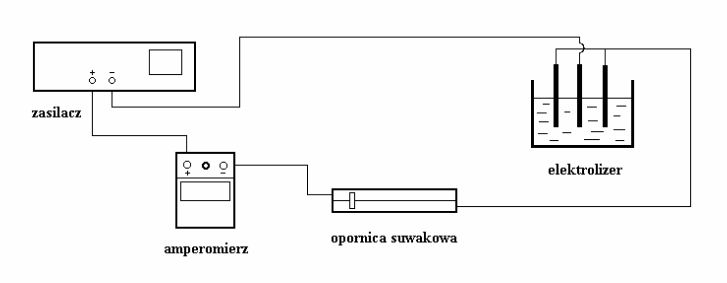
\includegraphics[width=1\textwidth]{img/elektroliza.png} 
	\captionsource{Schemat obwodu elektrycznego do przeprowadzenia elektrolizy}{Instrukcja do doświadczenia}
	\label{fig:img1}
\end{figure}

Doświadczenie rozpoczęliśmy od oczyszczenia miedzianych elektrod przy pomocy wody destylowanej i papieru ściernego. Po dokładnym osuszeniu, każda z nich została zważona osobno na wadze elektronicznej.

Następnie wszystkie elementy zostały podłączone w układ jak przedstawiono na schemacie (Rys. \ref{fig:img1}). Do katody podpięty został zacisk ,,-'' zasilacza, a do dwóch anod zaciski ,,+''. Po zanurzeniu elektrod w roztworze \ce{CuSO4}, włączyliśmy zasilacz, dostosowaliśmy napięcie zasilacza, aby amperomierz wskazywał $0,5$~A i włączyliśmy stoper. 

Podczas procesu elektrolizy, trwającego $30$~min, korygowaliśmy napięcie zasilacza, aby amperomierz stale wskazywał $0,5$~A. Po upływie czasu trwania doświadczenia, wyłączyliśmy zasilanie, wyciągnęliśmy elektrody z zacisków i delikatnie oczyściliśmy wodą destylowaną z resztek roztworu soli. Następnie dokładnie osuszyliśmy każdą z elektrod i zważyliśmy.

% OPRACOWANIE DANYCH POMIAROWYCH
\section{Opracowanie danych pomiarowych}
\subsection{Pomiary}

Czas trwania elektrolizy wynosił $t = (1800 \pm 1)$~s. Niepewność $u(t)$ szacujemy na $1$~s, ze względu na refleks eksperymentatorów przy włączaniu i wyłączaniu stopera.

Natężenie prądu wynosi $I = (500,00 \pm 0,17)$~mA, gdzie $u(I)$ zostało wyliczone ze wzoru:
\begin{equation}
	u(I) = \frac{1}{\sqrt{3}}~\frac{k}{100} z,
\end{equation}
gdzie $z$ to zakres amperomierza, a $k$ jego klasa. We wzorze występuje dzielenie przez $\sqrt{3}$, aby uzyskać niepewność standardową (co zalecane jest w przypadku urządzeń analogowych).
\pagebreak

\begin{table}[!ht]
	\caption{Masy elektrod przed i po elektrolizie wraz z różnicą mas}
	\centering
	\begin{tabular}{l|c|c|c}
		\hline Elektroda & Masa przed [g] & Masa po [g] & Różnica mas [g] \\ \hline \hline
		Katoda & $113,905$ & $114,223$ & $0,318$ \\
		Anoda 1 & $61,450$ & $61,285$ & $0,165$ \\
		Anoda 2 & $76,876$ & $76,736$ & $0,140$ \\ \hline
	\end{tabular}
	\label{tab:tab1}
\end{table}

W tabeli powyżej znajdują się masy elektrod w kolejnych etapach doświadczenia. Różnica masy katody wynosi $m_K = 318$~mg, a suma różnic mas anod wynosi $m_A = 165 + 140 = 305$~[mg]. Masę wytrąconej miedzi $m_{\ce{Cu}}$ przyjmujemy jako średnią arytmetyczną $m_K$ i $m_A$, a niepewność tego pomiaru jako $u(m_{\ce{Cu}}) = 0.01$~g, uwzględniając możliwą utratę masy podczas przemywania elektrod.

Przekształcając wzór (\ref{eq:faraday1}) możemy obliczyć wartość równoważnika elektrochemicznego substancji:
\begin{equation}
	k = \frac{m}{It}.
	\label{eq:k}
\end{equation}
Dla uproszczenia obliczeń kolejnych niepewności będziemy rozważać niepewność względną pomiaru $k$:
\begin{equation}
	\frac{u(k)}{k} = \sqrt{\Bigg(\frac{u(m)}{m}\Bigg)^2 + \Bigg(\frac{u(I)}{I}\Bigg)^2 + \Bigg(\frac{u(t)}{t}\Bigg)^2}.
	\label{eq:k_rel}
\end{equation}
Ze wzorów (\ref{eq:k}) i (\ref{eq:k_rel}) otrzymujemy wartość $k = (0,346 \pm 0,011)~\frac{\textrm{mg}}{\textrm{C}}$.

Wartość stałej Faradaya liczymy z przekształconego wzoru (\ref{eq:faraday2}):
\begin{equation}
	F = \frac{\mu}{wk}.
	\label{eq:F}
\end{equation}
Niepewność względna pomiaru stałej Faradaya opisana jest wzorem:
\begin{equation}
	\frac{u(F)}{F} = \frac{u(k)}{k}.
	\label{eq:F_rel}
\end{equation}
Dla \ce{CuSO4} odczytujemy $\mu = 63,58~\frac{\textrm{g}}{\textrm{mol}}$ oraz $w = 2$ i zakładamy, że  są to wartości tabelaryczne. Ze wzorów (\ref{eq:F}) i (\ref{eq:F_rel}) mamy $F = (91849 \pm 2900)$~C.

Wartość ładunku elementarnego liczymy z przekształconego wzoru (\ref{eq:faraday3}):
\begin{equation}
	e = \frac{F}{N_A},
	\label{eq:e}
\end{equation}
gdzie $N_A = 6,0245 \cdot 10^{23}~\frac{\textrm{g}}{\textrm{mol}}$.
Niepewność względna ładunku elementarnego przyjmuje postać:
\begin{equation}
	\frac{u(e)}{e} = \frac{u(k)}{k}.
	\label{eq:e_rel}
\end{equation}

Ze wzorów (\ref{eq:e}) i (\ref{eq:e_rel}) mamy $e = (0,1524 \pm 0,0048)$~aC.

\begin{table}[!ht]
	\caption{Zestawienie otrzymanych wartości $k$, $F$ i $e$ oraz ich niepewności}
	\centering
	\begin{tabular}{l|c|c|c|c|c}
		\hline & Wartość & Wartość & Różnica & Niepewność & Niepewność \\ 
		& tabelaryczna & obliczona &  & bezwzględna & względna [\%] \\ \hline \hline
		$k~\big[\frac{\textrm{mg}}{\textrm{C}}\big]$ & $0,3294$ & $0,346$ & $0,0166$ & $0,011$ & $3,2$   \\
		$F$~[C] & $96500$ & $91849$  & $4650$ & $2900$ & $3,2$ \\
		$e$~~[aC] & $0,1602$ & $0,1524$ & $ 0,0078$ & $0,0048$ & $3,2$ \\ \hline
	\end{tabular}
	\label{tab:tab2}
\end{table}

\subsection{Analiza wyników}

Niepewność rozszerzona pomiaru wartości równoważnika elektrochemicznego dla \ce{CuSO4} wynosi $U(k) = 0,022~\frac{\textrm{mg}}{\textrm{C}}$.
Dla uzyskanej wartości różnicy $\Delta k$ mamy nierówność:
\begin{equation}
	\Delta k = 0,0166 < U(k) = 0,22~\Big[\frac{\textrm{mg}}{\textrm{C}}\Big],
\end{equation}
z której wynika, że uzyskana wartość $k$ jest zgodna z wartością tabelaryczną.

Niepewność rozszerzona pomiaru wartości stałej Faradaya jest równa $\\U(F) = 5800$~C.
Dla uzyskanej wartości różnicy $\Delta F$ mamy nierówność:
\begin{equation}
\Delta F = 4650 < U(F) = 5800~[\textrm{C}],
\end{equation}
z której wynika, że uzyskana wartość $F$ jest zgodna z wartością tabelaryczną.

Niepewność rozszerzona pomiaru wartości ładunku elementarnego wynosi $U(e) = 0,0096$~aC.
Dla uzyskanej wartości różnicy $\Delta e$ mamy nierówność:
\begin{equation}
\Delta e = 0,0078 < U(e) = 0,0096~[\textrm{aC}],
\end{equation}
z której wynika, że uzyskana wartość $e$ jest zgodna z wartością tabelaryczną.

\section{Wnioski}

Wszystkie wyznaczone wartości doświadczalne były zgodne z odpowiadającymi im wartościami tabelarycznymi. Możemy więc stwierdzić, że podczas przeprowadzania doświadczenia nie zostały popełnione błędy gruby i systematyczny.

Aniony \ce{SO4^{2-}} reagowały z miedzianą anodą tworząc sól \ce{CuSO4}. W konsekwencji stężenie soli w roztworze nie zmieniało się. Wskazują na to otrzymane wartości różnicy mas elektrod po doświadczeniu i zgodność wartości stałej Faradaya z jej wartością tabelaryczną. Na podstawie wyników tego doświadczenia jesteśmy w stanie potwierdzić \textit{Prawo zachowania masy}.

\end{document}
